\documentclass[conference]{IEEEtran}
\IEEEoverridecommandlockouts
\usepackage{cite}
\usepackage{amsmath,amssymb,amsfonts}
\usepackage{algorithmic}
\usepackage{graphicx}
\usepackage{textcomp}
\usepackage{xcolor}
\usepackage{booktabs}
\def\BibTeX{{\rm B\kern-.05em{\sc i\kern-.025em b}\kern-.08em
    T\kern-.1667em\lower.7ex\hbox{E}\kern-.125emX}}

% ---------------------------------------------------------------
% PLACEHOLDER MACRO  --  DRAFT / SUBMISSION SWITCH
%
% \PH{...} marks an editorial note to the authors. Notes are NOT part
% of the paper's argument: every sentence reads correctly with them
% hidden.
%
%   \draftmodetrue   -> notes printed in red   (working draft)
%   \draftmodefalse  -> notes hidden entirely  (SUBMISSION)
%
% SET THIS TO \draftmodefalse BEFORE GENERATING THE SUBMISSION PDF.
% ---------------------------------------------------------------
\newif\ifdraftmode
\draftmodetrue
\ifdraftmode
  \newcommand{\PH}[1]{\textcolor{red}{[\,#1\,]}}
\else
  \newcommand{\PH}[1]{}
\fi

% ---------------------------------------------------------------
% CLICKABLE CROSS-REFERENCES
% hyperref must be loaded LAST. It turns every \cite, \ref and DOI
% into a live link: clicking [2] jumps to reference 2.
% For camera-ready submission, swap the options below for
%   \usepackage[hidelinks]{hyperref}
% which keeps the links active but prints them in plain black.
% ---------------------------------------------------------------
% Define consistent link color without commas in \usepackage options
\definecolor{linkblue}{rgb}{0,0,0.6}
\usepackage[colorlinks=true,
            linkcolor=linkblue,
            citecolor=linkblue,
            urlcolor=linkblue,
            breaklinks=true]{hyperref}

\begin{document}

\title{The Effect of XAI Explanation Types on User Trust\\ and Purchase Intention in a Conversational\\ Recommender System for the Perfume Domain}

% ---------------------------------------------------------------
% DOUBLE-BLIND SUBMISSION
% Author identities are withheld for review. Before the camera-ready
% version, restore the real author block here and also restore the
% institution name in Section IV.B (currently anonymised there too).
% ---------------------------------------------------------------
\author{\IEEEauthorblockN{1\textsuperscript{st} Given Name Surname}
\IEEEauthorblockA{\textit{dept. name of organization (of Aff.)} \\
\textit{name of organization (of Aff.)}\\
City, Country \\
email address or ORCID}
\and
\IEEEauthorblockN{2\textsuperscript{nd} Given Name Surname}
\IEEEauthorblockA{\textit{dept. name of organization (of Aff.)} \\
\textit{name of organization (of Aff.)}\\
City, Country \\
email address or ORCID}
\and
\IEEEauthorblockN{3\textsuperscript{rd} Given Name Surname}
\IEEEauthorblockA{\textit{dept. name of organization (of Aff.)} \\
\textit{name of organization (of Aff.)}\\
City, Country \\
email address or ORCID}
}

\maketitle

\begin{abstract}
Explanations are widely assumed to increase user trust in AI-based recommender systems,
yet the effect depends on the kind of explanation given rather than on its presence.
Comparative evidence on explanation types is scarce in conversational recommender systems
and almost absent in sensory-hedonic domains, where the defining product attribute cannot
be conveyed through a screen. This paper reports a between-subjects experiment with 90
participants, 30 per condition, conducted in a physical perfume store with an agent in
which a large language model handles dialogue while a knowledge-graph embedding backend
selects the items. Three justification logics were set by system-prompt conditioning:
feature-based, narrative-based, and comparative-based. Justification logic significantly
affected both perceived trust and purchase intention, with a large and a medium-to-large
effect respectively. Contrary to the design intuition that warmer explanations build
trust, narrative justification produced the lowest trust, whereas comparative
justification produced the highest purchase intention. Trust and purchase intention were
only weakly associated (Spearman rho = 0.229, p = 0.030), and no evidence of moderation by
perfume familiarity was found. Because trust was jointly highest under feature-based and
comparative justification while purchase intention was highest under comparative
justification alone, the two design objectives are not served by the same condition. What
governs the response appears to be the evaluative nature of the user's task rather than
the hedonic nature of the product.
\end{abstract}

\begin{IEEEkeywords}
explainable AI, conversational recommender systems, user behavior analysis, user
experience evaluation, perceived trust, purchase intention, hedonic domain
\end{IEEEkeywords}

% ===============================================================
\section{Introduction}
% ===============================================================

Conversational recommender systems (CRS) support a multi-turn dialogue in which the system
elicits preferences, explains its suggestions, and processes feedback \cite{jannach2021}.
Large language models (LLMs) have made such systems inexpensive to build, sharpening a
question that predates them: when a recommender explains itself, what should it say? This
paper answers that question empirically, through user behaviour analysis rather than
algorithmic contribution.

Explainable AI (XAI) is positioned as the bridge between opaque models and users deciding
how far to rely on them \cite{rong2024}. Explanations may serve seven aims, including
transparency, trust, and persuasiveness, and these can be incompatible, so an explanation
optimised for one may degrade another \cite{tintarev2012}. Consumer research supports the
optimistic half: post hoc explanations raise interpretability perceptions and thence trust,
purchase intention, and click-through \cite{chen2024}. The pessimistic half receives less
attention. Feature-importance explanations produced higher trust than counterfactual ones,
and explanations raised trust even when the system performed poorly, which the authors read
as overreliance rather than warranted trust \cite{brito2023}; explanation interfaces can
likewise induce trust calibration errors \cite{naiseh2021}. The question therefore shifts
from whether an explanation is present to which kind is given.

Two gaps follow. Explanation types are seldom compared against one another inside a single
conversational system: the demonstration that explanation type determines which component
of trust is affected used a static recommendation agent \cite{wang2007}, and later
comparisons of feature-importance against counterfactual explanation \cite{brito2023}, or
taxonomies of contrastive generation \cite{stepin2021}, sit outside conversational
e-commerce. Sensory-hedonic domains also remain underexplored, which matters because the
effect of explanation is not domain invariant: it is stronger in utilitarian domains, and
explanation type interacts with domain \cite{chen2024}. Negative reviews likewise depress
purchase for utilitarian but not hedonic products \cite{varga2024}, and product type
moderates the path from perceived deception to repurchase intention \cite{wangx2022}.
Perfume is an extreme case: its defining attribute cannot be transmitted digitally at all,
its vocabulary is mastered mainly by enthusiasts, and online purchase uncertainty is
correspondingly high.

Three questions follow. \textbf{RQ1:} Does justification logic affect perceived trust and
purchase intention? \textbf{RQ2:} Is trust associated with purchase intention?
\textbf{RQ3:} Does familiarity moderate the effect?

This paper contributes a perfume CRS in which an LLM handles language while a
knowledge-graph embedding backend selects items, with justification logic switched by
system-prompt conditioning; comparative evidence in a domain whose core attribute is not
digitally transmissible \cite{chen2024}; a counter-intuitive result, that narrative
justification produced the \textit{lowest} trust, consistent with evidence that competent
conversational styles outperform warm ones on cognition-oriented tasks \cite{libaoku2024};
and an explicit design trade-off, since the conditions maximising trust and purchase
intention differ.

% ===============================================================
\section{Related Work}
\label{sec:related}
% ===============================================================

\subsection{Explanation Types and Trusting Beliefs}

That explanation type matters, and not merely explanation presence, was settled on a static
recommendation agent: \textit{how} explanations raised competence and benevolence beliefs,
\textit{why} explanations benevolence, and \textit{trade-off} explanations integrity
\cite{wang2007}. Tintarev and Masthoff sharpened the point from the opposite direction,
finding that personalising feature-based explanations was \textit{detrimental} to
effectiveness while plausibly improving satisfaction, contrary to their own hypothesis
\cite{tintarev2012}. Recent comparisons pit feature-importance against counterfactual
explanation, with the former yielding higher trust among non-experts and, more
uncomfortably, explanations raising trust even in an unreliable system \cite{brito2023};
contrastive generation methods have been organised into a taxonomy \cite{stepin2021}; and
design principles have been proposed that target trust calibration rather than trust
maximisation \cite{naiseh2021}. A review of 97 user studies concludes that XAI
effectiveness is not consistent across applications \cite{rong2024}. None of this work,
however, places two or more explanation types side by side inside a single multi-turn
conversational system; the comparisons are made on static displays or outside e-commerce.

\subsection{Explanations in Conversational Recommenders}

Jannach et al. note that although explanations are considered central to a convincing
dialogue, the topic is not explored a great deal \cite{jannach2021}. What has been explored
is the container rather than the content. Interactive conversational explanation improves
user evaluation when users can scrutinise the explanatory arguments \cite{ziegler2023}, and
dialogue aspects shaping satisfaction have been annotated, with relevance dominant at turn
level \cite{siro2023}. The closest methodological parallel built three CRS versions and ran
a between-subjects experiment with 66 participants, finding no significant effect on any
questionnaire-based construct although objective measures differed \cite{ziegfeld2025} ---
but that manipulation concerned how preferences were elicited, not how recommendations were
justified.

\subsection{Trust, Anthropomorphism, and Purchase Intention}

Trust in an artefact is conventionally decomposed into competence, benevolence, and
integrity \cite{mcknight2002}, and user-centric evaluation supplies validated constructs
along with the guidance that explaining \textit{why} increases transparency while
explaining \textit{trade-offs} increases persuasion \cite{pu2012}. The trust-to-purchase
chain has been validated for chatbots using questionnaires and EEG, though neither media
richness nor playfulness raised trust, the authors reasoning that shopping conversation is
a functional task \cite{yen2021}. Anthropomorphism qualifies the chain: exchange
relationships strengthen the weight of competence over warmth \cite{cheng2022}; warmth and
competence feed both trust and chatbot overload, so trust is not the sole route to purchase
\cite{liyang2025}; anthropomorphism can backfire through expectancy violation
\cite{crolic2022}; and no interaction style is universally superior, competent styles
winning cognition-oriented tasks and warm styles emotion-oriented ones \cite{libaoku2024}.
These findings concern conversational \textit{style}, however, and leave the content of the
justification fixed.

\subsection{Hedonic Domains and Domain Familiarity}

Hedonic evaluation is subjective and unstable relative to utilitarian evaluation
\cite{wangx2022}, \cite{varga2024}. The anchor study for this work establishes that post hoc
explanations raise interpretability and thence trust, that the effect is stronger in
utilitarian domains, and that attribute-based explanations suit utilitarian domains while
user-based ones suit hedonic domains \cite{chen2024}. Familiarity is a plausible boundary
condition, since expertise reduces trust in explainable decision support and moderates the
effect of explanation on trusting intention \cite{bayer2023}, an interaction that required
four experiments and 731 participants to characterise \cite{celar2023}. What has not been
tested is whether these domain effects survive in conversation, and no comparative test of
explanation type exists in an olfactory setting.

The three gaps intersect at a single untested case. This study compares three justification
logics against one another rather than against a no-explanation baseline, inside a
multi-turn LLM-driven conversation rather than on a static display, in a domain whose
defining attribute cannot be conveyed by the interface at all.

% ===============================================================
\section{Methodology}
\label{sec:method}
% ===============================================================

\subsection{System Architecture}

The platform is a conversational perfume recommender deployed as a web application and
operated on site in a physical perfume store. GPT-4o-mini conducts the dialogue, extracts
preferences, and verbalises the justification, while a conversational-recommendation hybrid
knowledge graph embedding (CR-HKGE) backend selects the items (Fig.~\ref{fig:arch}).

\begin{figure}[htbp]
\centerline{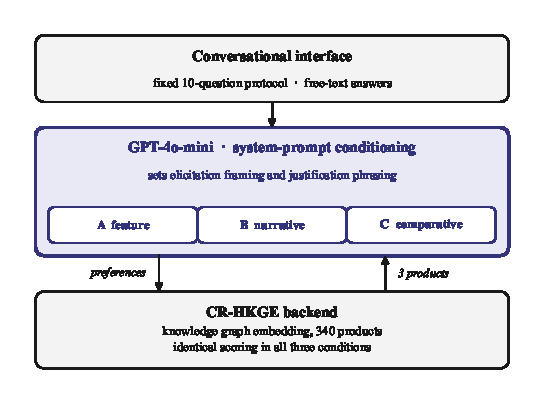
\includegraphics[width=0.92\columnwidth]{fig_architecture}}
\caption{System architecture. Item selection is delegated to the backend, whose scoring is
identical in every condition; the condition is set once, at the system-prompt layer, and
governs both elicitation and justification.}
\label{fig:arch}
\end{figure}

This separation is the design decision on which the experiment rests. First, \textit{the
backend is a knowledge graph embedding model, not a retrieval-augmented generation
pipeline}: candidates are scored in a learned embedding space over a graph of 998 entities
and 9,255 triples across seven relation types, including 340 catalogue products, so
selecting three items is a non-trivial retrieval problem. The approach follows
knowledge-graph recommenders that aggregate collaborative and semantic signals through
graph attention \cite{litois2023}, including work extending such graphs to conversational
settings to capture a user's situation and emotional state \cite{yang2025}. Second,
\textit{the LLM is an interface, not the recommender}, mirroring the pattern that employs
LLMs as the brain and recommender models as tools \cite{huang2023}, motivated by the
observation that LLMs lack knowledge of domain-specific catalogues and propose products
that do not exist. The recommendation \textit{algorithm} is therefore invariant across
conditions; the recommended \textit{items} are not, since the backend is queried with a
preference record the dialogue itself produces.

\subsection{The Three Justification Logics}

The condition is fixed by system-prompt conditioning at the start of each session, without
fine-tuning, following the prompting paradigm by which LLMs are adapted to recommendation
tasks \cite{zhao2024}. Table~\ref{tab:conditions} specifies the three conditions.

\begin{table*}[htbp]
\caption{The Three Experimental Conditions}
\begin{center}
\renewcommand{\arraystretch}{1.15}
\begin{tabular}{@{}p{0.5cm}p{2.0cm}p{1.5cm}p{5.4cm}p{5.6cm}@{}}
\toprule
& \textbf{Condition} & \textbf{Logic} & \textbf{Elicitation framing (parallel item)} & \textbf{Explanation content} \\
\midrule
A & Feature-based & Attributive & ``Do you prefer something dominantly fresh such as citrus, something warm such as woody, or something floral?'' & Names the olfactory family and main accords, tying each to a stated preference. Cross-referencing is forbidden. \\
B & Narrative-based & Affective & ``When you wear this later, how do you want to feel --- more confident, calmer, or freer?'' & Connects the scent to a moment, mood, or identity. Technical vocabulary and cross-referencing are forbidden. \\
C & Comparative-based & Contrastive & ``Fresh and light like morning air, versus warm and deep like wood --- which are you closer to?'' & Positions each product against at least one other, translating technical terms into comparative language. \\
\bottomrule
\end{tabular}
\label{tab:conditions}
\end{center}
\footnotesize\textit{Note.} Elicitation examples are translated from the Indonesian
prompts. The agent is forbidden to disclose which style it is using.
\end{table*}

Each condition operationalises a claim from the literature. Condition A instantiates
attribute-based explanation, chosen because feature-importance explanations yield higher
trust than counterfactual ones among non-expert users \cite{brito2023}. Condition C
instantiates contrastive explanation \cite{stepin2021}, chosen because contrastive
information improves the accuracy of users' \textit{own} decisions \cite{celar2023} --- the
capability a buyer needs when the decisive attribute cannot be conveyed by the interface.
Condition B exists precisely because the literature has not tested it: work on warmth and
competence manipulates conversational style \cite{libaoku2024}, \cite{cheng2022} while
treating explanation content as fixed. Condition B instead makes affective content the
substance of the justification, supplying no compositional facts and no comparative frame.
It is closest to the user-based explanations found more effective in hedonic domains
\cite{chen2024}, differing in one respect examined later: user-based explanations carry
social proof, purely narrative ones carry none.

The manipulated variable is therefore the \textit{justification logic}, and each prompt
instructs the agent to hold its assigned logic ``from your first greeting to your final
closing message,'' so the ten elicitation questions are framed differently in each
condition, as is the final explanation. This is deliberate --- a system whose framing
contradicted its own explanations would be incoherent --- but its cost is that explanation
content cannot be separated from conversational framing. The contrast is visible in how the
logics render the same product: A produced ``\textit{it belongs to the aquatic family with
green and fresh-spicy as its main character}''; B, ``\textit{picture a fresh scent flowing
gently, like morning dew}''; C, ``\textit{it is the freshest of the three}''. One asymmetry
bears on a later analysis: the closing messages in A and C invite the user to smell the
fragrances at the tester area, whereas B does not.

\subsection{Design, Participants, and Procedure}

The study uses a single-factor between-subjects design with three levels of justification
logic, assignment by session counter, and 30 participants per condition. Had participants
experienced all three logics the comparison would have become explicit, inviting demand
characteristics and carryover; the cost of avoiding this is reduced power for the
interaction test.

Familiarity was recorded at the first elicitation question and recruitment was
quota-balanced across its three levels: 30 beginners, 30 enthusiasts, 30 collectors. These
were dichotomised for analysis, beginners coded \textit{novice} ($n = 30$) and enthusiasts
with collectors coded \textit{enthusiast} ($n = 60$), on the ground that what separates the
groups is command of olfactory vocabulary, on which condition A rests entirely. The
two-to-one imbalance therefore follows from the coding decision rather than recruitment,
though the novice cells are small --- 10, 12, and 8. Familiarity was nonetheless evenly
distributed, $\chi^{2}(2) = 1.200$, $p = .549$, Cram\'{e}r's $V = 0.116$.

A session proceeds through greeting and consent, elicitation, presentation of three ranked
perfumes with the condition-appropriate explanation, and the questionnaire. Elicitation
follows a fixed protocol of exactly ten questions, one per message: in the terms of Ziegfeld
et al. \cite{ziegfeld2025} this is the \textit{high-guidance, low-restriction} point of the
elicitation space. Sessions comprised a mean of 20.29 messages ($SD = 4.67$, range 9--55),
with means of 20.60 in A, 19.20 in B, and 21.07 in C, so interaction length is an unlikely
alternative explanation for the differences reported below. Because the tester area remained
accessible, participants could smell the recommended fragrances physically.

Age and gender were not recorded. Participation was voluntary and preceded by an on-screen
consent notice stating that the system formed part of collaborative academic research at
the authors' institution, that responses would be anonymised, and that participation could
be declined. No personally identifying information was collected and no compensation was
offered. The study involved no deception beyond withholding the research hypothesis, no
sensitive data, and no vulnerable population. It was not submitted for formal institutional
ethics review.

\subsection{Measures and Analysis Plan}

Four constructs were measured with two five-point Likert items each, administered in
Indonesian: trust, whether the recommended perfumes matched the participant's preferences
and whether the explanation convinced them the system understood their needs
\cite{mcknight2002}; purchase intention and satisfaction, adapted from the ResQue framework
\cite{pu2012}; and usefulness, whether the explanation clarified why the perfume suited them
and supported their decision \cite{davis1989}. A ninth, binary item recorded whether the
participant had already smelled the recommended product, measuring sensory access already
obtained rather than an intention to obtain it.

To verify that conditions were distinguishable from transcripts alone, 30 transcripts, 10
per condition, were coded by three sources: the system-recorded condition, the researcher,
and an independent rater blind to assignment. Agreement was quantified with Cohen's kappa
against the benchmarks of Landis and Koch, who assign 0.81--1.00 to almost perfect agreement
while noting the divisions are arbitrary \cite{landis1977}. Because self-coding was not
blind, evidentiary weight rests on the independent rater.

Cronbach's alpha is downward-biased for two-item scales, so reliability was estimated with
the Spearman-Brown coefficient \cite{eisinga2013}. Shapiro-Wilk tests indicated departures
from normality in several cells and Levene's test heterogeneity of variance for trust, so
rank-based procedures were adopted: Kruskal-Wallis, Dunn's test with Holm correction,
Spearman's rho, and Wilcoxon signed-rank. Effect size was computed as
$\varepsilon^{2} = H/(n-1)$, with rank-biserial correlations for pairwise comparisons. The
moderation hypothesis used a two-way analysis of variance, an acknowledged inconsistency
adopted for want of an established rank-based test of a two-factor interaction. Analyses
used JASP v0.97.1.

% ===============================================================
\section{Result and Discussion}
\label{sec:results}
% ===============================================================

\subsection{Manipulation Check and Reliability}

The independent rater reproduced the system-recorded condition with $\kappa = 0.900$
($SE = 0.068$, 95\% CI [0.767, 1.000]); the researcher's own, non-blind coding matched
ground truth exactly. Both disagreements occurred in condition B, where the rater classified
narrative transcripts as feature-based. The manipulation was therefore not perfectly pure,
and its impurity ran towards condition A --- a direction that works \textit{against} the
effect reported below, making it a conservative estimate.

Spearman-Brown coefficients were 0.801 for purchase intention, 0.731 for usefulness, 0.689
for satisfaction, and 0.624 for trust (95\% CI [0.306, 0.941]). The trust figure is below
the conventional 0.70 threshold and reported unadjusted. Two features qualify it: the
interval is wide, reflecting the precision obtainable from two items and 90 observations,
and an inter-item correlation of 0.454 lies within the range considered healthy for a narrow
construct, indicating the constraint is scale length rather than item content.

\subsection{Results}

Trust was highest in condition C ($M = 4.65$, $SD = 0.35$) and lowest in B ($M = 4.05$,
$SD = 0.64$), with A intermediate ($M = 4.48$, $SD = 0.46$). Purchase intention was highest
in C ($M = 4.23$, $SD = 0.52$) against A ($M = 3.78$, $SD = 0.77$) and B ($M = 3.55$,
$SD = 0.84$). Usefulness and satisfaction were uniformly high in every condition, with means between
4.33 and 4.85, and both exceeded the 3.5 reference value decisively (Wilcoxon: $V = 3909$
and $V = 3533$, both $p < .001$), so the trust differences cannot be attributed to one
condition being served by a system that simply worked less well. Shapiro-Wilk tests
rejected normality in nine of the twelve construct-by-condition cells, and Levene's test
indicated heterogeneity of variance for trust, $F(2, 87) = 3.292$, $p = .042$.

\begin{figure}[htbp]
\centerline{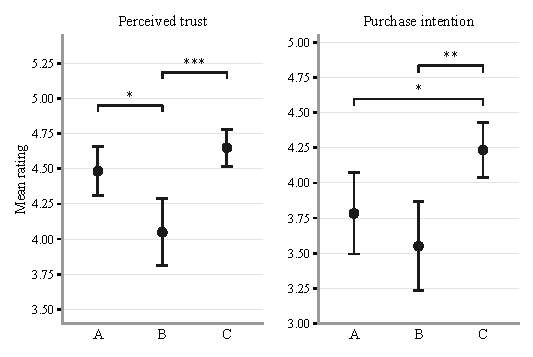
\includegraphics[width=0.94\columnwidth]{fig_means}}
\caption{Perceived trust and purchase intention by condition. Points are means with 95\%
confidence intervals; brackets mark Holm-corrected Dunn comparisons
($^{*}p<.05$, $^{**}p<.01$, $^{***}p<.001$).}
\label{fig:means}
\end{figure}

Condition affected perceived trust with a large effect ($\varepsilon^{2} = 0.186$). Dunn's
test located the difference: B scored below A ($z = 2.713$, $p = .013$) and below C
($z = -3.985$, $p < .001$), while A and C did not differ ($z = -1.272$, $p = .203$).
Condition also affected purchase intention ($\varepsilon^{2} = 0.133$), with C above A
($z = -2.326$, $p = .040$) and above B ($z = -3.365$, $p = .002$) while A and B did not
differ ($z = 1.039$, $p = .299$). The two patterns do not coincide: trust was jointly
highest in A and C, purchase intention highest in C alone. Trust and purchase intention were
positively but weakly associated ($\rho = 0.229$, 95\% CI [0.025, 0.437]); the parametric
counterpart did not reach significance, $r = 0.161$, $p = .129$. No evidence of interaction
between condition and familiarity was found, although the condition main effect persisted,
$F(2, 84) = 10.57$, $p < .001$. Table~\ref{tab:hyp} summarises.

\begin{table}[htbp]
\caption{Summary of Hypothesis Tests}
\begin{center}
\renewcommand{\arraystretch}{1.1}
\setlength{\tabcolsep}{3.4pt}
\begin{tabular}{@{}p{0.5cm}p{2.35cm}p{1.75cm}p{0.95cm}p{1.35cm}@{}}
\toprule
& \textbf{Test} & \textbf{Statistic} & \textbf{Effect} & \textbf{Outcome} \\
\midrule
H1 & Kruskal-Wallis, Dunn & $H(2)=16.57$, $p<.001$ & $\varepsilon^{2}=.186$ & Supported; B $<$ A, C \\
H2 & Kruskal-Wallis, Dunn & $H(2)=11.88$, $p=.003$ & $\varepsilon^{2}=.133$ & Supported; C $>$ A, B \\
H3 & Spearman & $\rho=.229$, $p=.030$ & CI [.025, .437] & Supported, weak \\
H4 & Two-way ANOVA & $F(2,84)=0.45$, $p=.638$ & --- & No evidence \\
\bottomrule
\end{tabular}
\label{tab:hyp}
\end{center}
\end{table}

Finally, 77 of 90 participants (85.6\%) had already smelled the recommended product, a
proportion that did not differ across conditions.

\subsection{Why Narrative Justification Lowered Trust}

The warmest justification was trusted least, in the direction opposite to the intuition
that motivated condition B. The most economical account is that emotional narrative weakens the signal of competence.
Li et al. show that no anthropomorphic style is universally superior: competent styles
produce more positive responses on cognition-oriented tasks, mediated by agent-mind
perception, whereas warm styles prevail on emotion-oriented tasks \cite{libaoku2024}. The
decisive variable is the nature of the \textit{task}, not of the \textit{product}. Perfume
is hedonic as a product, but selecting one through a recommender is an evaluative task: the
user weighs options, assesses fit, and decides. Two results converge. Exchange relationships
strengthen the weight of perceived competence on trust \cite{cheng2022}, and an in-store
consultation is an exchange relationship in the plainest sense; and neither media richness
nor playfulness raised trust in shopping chatbots, on the reasoning that such communication
is a functional task \cite{yen2021}. That anthropomorphic warmth can backfire outright,
through expectancy violation, is separately established \cite{crolic2022}.

The finding stands in apparent tension with the anchor study, which reports user-based
explanations as more effective in hedonic domains \cite{chen2024}. Two differences reconcile
the accounts. Their explanations accompany a static display, whereas ours are sustained
across a ten-question dialogue; in conversation the user accumulates evidence about the
system's competence, not only about the product, and a narrative that reads as evocative
once can read as evasive over twenty messages. Further, the two are not the same object:
user-based explanation carries social proof, purely narrative explanation carries no
evidence at all. Seen thus the result is less exotic than it appears, since personalising
explanations has previously been found detrimental to effectiveness even while improving
satisfaction \cite{tintarev2012}. Feature-based and comparative justification did not differ
on trust: both anchor the recommendation in something checkable, so either displays command
of the domain, which is what an evaluative task rewards \cite{brito2023}, \cite{wang2007}.

\subsection{A Thin Bridge to Purchase Intention}

The association was weak and the parametric coefficient non-significant, so no causal claim
is made. The more informative evidence is structural: were trust the principal route,
condition A should have followed C upward on purchase intention. It did not. Comparative
justification therefore appears to act through a channel that bypasses trust, most plausibly
by reducing decision uncertainty at the point of choice. Celar and Byrne provide direct support: counterfactual explanations
improved the accuracy of participants' \textit{own} decisions more than causal ones
\cite{celar2023}. Contrastive information helps people decide for themselves, which is what
is needed when the decisive attribute cannot be conveyed by the interface. This fits models
treating trust as one channel among several \cite{liyang2025} and qualifies the
trust-centric reading of the chatbot literature \cite{yen2021}; maximal trust is in any case
not the goal \cite{naiseh2021}.

The interaction with familiarity was far from significant, which is an absence of evidence
rather than evidence of absence. The grounds for expecting moderation were strong
\cite{bayer2023}, but the novice cells held 10, 12, and 8 participants, too few to detect a
plausible interaction, whereas characterising this interaction elsewhere required four
experiments and 731 participants \cite{celar2023}.

\subsection{Implications}

Three theoretical implications follow. First, the account above generalises: where the
literature partitions domains into utilitarian and hedonic \cite{chen2024},
\cite{wangx2022}, \cite{varga2024}, these results suggest a cross-cutting axis, whether the
user's immediate activity is evaluative or experiential. Second, they give concrete support
to the claim that explanatory aims can be incompatible \cite{tintarev2012}: the conditions
maximising trust and purchase intention differed. Third, a comparable three-condition CRS
study found no significant effect on any subjective construct while manipulating preference
elicitation \cite{ziegfeld2025}; the contrast suggests, without establishing, that
justification logic is a stronger lever than elicitation method, consistent with XAI
effectiveness varying across applications \cite{rong2024}.

Practically, if the objective is trust, ground the justification in something checkable even
in a domain that feels emotional. If the objective is conversion, comparative justification
was strongest, reproducing the guideline that explaining why increases transparency while
explaining trade-offs increases persuasion \cite{pu2012}. The two objectives are not served
by the same design. One caveat guards against over-reading: usefulness and satisfaction were
high in all conditions, so B underperformed specifically on trust, not globally.

\subsection{Limitations}

Two limitations were introduced above: the manipulation governs the whole interaction, so
explanation content cannot be separated from conversational framing, and item equivalence
across conditions was not verified against session logs. Four others apply.
\textit{Measurement:} the two-item trust scale fell below the conventional threshold, and
although measurement error attenuates effects, so that H1 is plausibly conservative, a
multi-item instrument is needed; usefulness and satisfaction showed ceiling effects.
\textit{Statistical approach:} main analyses are rank-based while the moderation test is
parametric. \textit{Design asymmetry:} conditions A and C invited participants to the tester
area and B did not. \textit{Generalisation:} data come from one store, one brand, and 90
participants in a single country, with age and gender unrecorded, and sensory access was
near-universal, so conclusions describe users who \textit{could} smell the product.

% ===============================================================
\section{Conclusion}
\label{sec:conclusion}
% ===============================================================

Justification logic affects both perceived trust and purchase intention (RQ1): narrative
justification, designed to be the warmest, produced the lowest trust, while comparative
justification produced the highest purchase intention. Trust is only weakly associated with
purchase intention (RQ2), and comparative justification appears to raise it through a route
bypassing trust. No evidence of moderation by familiarity was found (RQ3), better read as a
limitation of power. The central lesson is that a product being hedonic does not make an
emotional justification the right one; what governs the response appears to be the nature of
the user's task. The second is that the two objectives are not served by the same condition,
so designers in sensory domains face a trade-off rather than a ranking.

Four directions follow. Holding elicitation constant while varying only the final
justification would separate explanation content from conversational framing. Measuring
trust dimensionally would convert the proposed mechanism into a falsifiable prediction, that
narrative justification depresses competence beliefs specifically while leaving benevolence
intact, for which the demonstration that explanation types engage different trusting beliefs
\cite{wang2007} supplies the instrument design. Hybrid conditions would establish whether
narrative functions as a complement rather than a substitute when attached to a factual
base, for which recommenders that capture situation and emotional state from dialogue
\cite{yang2025} offer a foundation and interactive explanation interfaces
\cite{ziegler2023} a means of letting users assemble the hybrid themselves. Finally,
replication across domains differing in digital transmissibility, with larger
familiarity-balanced samples and finer-grained dialogue measures \cite{siro2023}, would put
the task-based account at risk.


\begin{thebibliography}{00}
\setlength{\itemsep}{0pt}\setlength{\parskip}{0pt}

\bibitem{jannach2021}
D. Jannach, A. Manzoor, W. Cai, and L. Chen, ``A survey on conversational
recommender systems,'' \textit{ACM Comput. Surv.}, vol. 54, no. 4, Art. 105,
May 2021.

\bibitem{rong2024}
Y. Rong \textit{et al.}, ``Towards human-centered explainable AI: A survey of user
studies for model explanations,'' \textit{IEEE Trans. Pattern Anal. Mach. Intell.},
vol. 46, no. 4, pp. 2104--2122, Apr. 2024.

\bibitem{tintarev2012}
N. Tintarev and J. Masthoff, ``Evaluating the effectiveness of explanations for
recommender systems: Methodological issues and empirical studies on the impact of
personalization,'' \textit{User Model. User-Adapt. Interact.}, vol. 22, pp. 399--439, 2012.

\bibitem{chen2024}
C. Chen, A. D. Tian, and R. Jiang, ``When post hoc explanation knocks: Consumer
responses to explainable AI recommendations,'' \textit{J. Interactive Marketing},
vol. 59, no. 3, pp. 234--250, 2024.

\bibitem{brito2023}
R. de Brito Duarte, F. Correia, P. Arriaga, and A. Paiva, ``AI trust: Can
explainable AI enhance warranted trust?,'' \textit{Human Behav. Emerg. Technol.},
vol. 2023, Art. 4637678, 12 pages, 2023.

\bibitem{naiseh2021}
M. Naiseh, D. Al-Thani, N. Jiang, and R. Ali, ``Explainable recommendation: When
design meets trust calibration,'' \textit{World Wide Web}, vol. 24, pp. 1857--1884,
2021.

\bibitem{wang2007}
W. Wang and I. Benbasat, ``Recommendation agents for electronic commerce: Effects of
explanation facilities on trusting beliefs,'' \textit{J. Manage. Inf. Syst.},
vol. 23, no. 4, pp. 217--246, 2007.

\bibitem{stepin2021}
I. Stepin, J. M. Alonso, A. Catala, and M. Pereira-Fari\~{n}a, ``A survey of
contrastive and counterfactual explanation generation methods for explainable
artificial intelligence,'' \textit{IEEE Access}, vol. 9, pp. 11974--12001, 2021.

\bibitem{varga2024}
M. Varga and P. Albuquerque, ``The impact of negative reviews on online search and
purchase decisions,'' \textit{J. Marketing Res.}, vol. 61, no. 5, pp. 803--820,
2024.

\bibitem{wangx2022}
X. Wang, A. R. Ashraf, N. Thongpapanl, and K.-Y. Wang, ``Perceived deception and
online repurchase intention: The moderating effect of product type and consumer
regulatory orientation,'' \textit{J. Consumer Behav.}, vol. 21, no. 6,
pp. 1522--1539, 2022.

\bibitem{libaoku2024}
B. Li, R. Yao, and Y. Nan, ``How does anthropomorphism promote consumer responses to
social chatbots: Mind perception perspective,'' \textit{Internet Research},
vol. 35, no. 6, pp. 2471--2495, 2025.

\bibitem{ziegler2023}
D. C. Hernandez-Bocanegra and J. Ziegler, ``Explaining recommendations through
conversations: Dialog model and the effects of interface type and degree of
interactivity,'' \textit{ACM Trans. Interact. Intell. Syst.}, vol. 13, no. 2,
Art. 6, Apr. 2023.

\bibitem{siro2023}
C. Siro, M. Aliannejadi, and M. de Rijke, ``Understanding and predicting user
satisfaction with conversational recommender systems,'' \textit{ACM Trans. Inf.
Syst.}, vol. 42, no. 2, Art. 55, Nov. 2023.

\bibitem{ziegfeld2025}
L. Ziegfeld, D. Di Scala, and A. H. M. Cremers, ``The effect of preference
elicitation methods on the user experience in conversational recommender systems,''
\textit{Comput. Speech Lang.}, vol. 89, Art. 101696, 2025.

\bibitem{mcknight2002}
D. H. McKnight, V. Choudhury, and C. Kacmar, ``Developing and validating trust
measures for e-commerce: An integrative typology,'' \textit{Inf. Syst. Res.},
vol. 13, no. 3, pp. 334--359, 2002.

\bibitem{pu2012}
P. Pu, L. Chen, and R. Hu, ``Evaluating recommender systems from the user's
perspective: Survey of the state of the art,'' \textit{User Model. User-Adapt.
Interact.}, vol. 22, pp. 317--355, 2012.

\bibitem{yen2021}
C. Yen and M.-C. Chiang, ``Trust me, if you can: A study on the factors that
influence consumers' purchase intention triggered by chatbots based on brain image
evidence and self-reported assessments,'' \textit{Behav. Inf. Technol.}, vol. 40,
no. 11, pp. 1177--1194, 2021.

\bibitem{cheng2022}
X. Cheng, X. Zhang, J. Cohen, and J. Mou, ``Human vs. AI: Understanding the impact
of anthropomorphism on consumer response to chatbots from the perspective of trust
and relationship norms,'' \textit{Inf. Process. Manage.}, vol. 59, Art. 102940,
2022.

\bibitem{liyang2025}
Y. Li, Z. Gan, and B. Zheng, ``How do artificial intelligence chatbots affect
customer purchase? Uncovering the dual pathways of anthropomorphism on service
evaluation,'' \textit{Inf. Syst. Frontiers}, vol. 27, pp. 283--300, 2025.

\bibitem{crolic2022}
C. Crolic, F. Thomaz, R. Hadi, and A. T. Stephen, ``Blame the bot: Anthropomorphism
and anger in customer-chatbot interactions,'' \textit{J. Marketing}, vol. 86, no. 1,
pp. 132--148, 2022.

\bibitem{bayer2023}
S. Bayer, H. Gimpel, and M. Markgraf, ``The role of domain expertise in trusting and
following explainable AI decision support systems,'' \textit{J. Decision Syst.},
vol. 32, no. 1, pp. 110--138, 2023.

\bibitem{celar2023}
L. Celar and R. M. J. Byrne, ``How people reason with counterfactual and causal
explanations for artificial intelligence decisions in familiar and unfamiliar
domains,'' \textit{Memory \& Cognition}, vol. 51, pp. 1481--1496, 2023.

\bibitem{litois2023}
Y. Li, L. Hou, and J. Li, ``Preference-aware graph attention networks for
cross-domain recommendations with collaborative knowledge graph,'' \textit{ACM Trans.
Inf. Syst.}, vol. 41, no. 3, Art. 80, Feb. 2023.

\bibitem{yang2025}
H. Yang, D. Kim, G. Park, K. Yeom, and K.-H. Lee, ``CoreSense: Social commonsense
knowledge-aware context refinement for conversational recommender system,''
\textit{IEEE Trans. Knowl. Data Eng.}, vol. 37, no. 4, pp. 1702--1712, Apr. 2025.

\bibitem{huang2023}
X. Huang, J. Lian, Y. Lei, J. Yao, D. Lian, and X. Xie, ``Recommender AI agent:
Integrating large language models for interactive recommendations,'' \textit{ACM Trans.
Inf. Syst.}, vol. 43, no. 4, Art. 96, 33 pages, 2025.

\bibitem{zhao2024}
Z. Zhao \textit{et al.}, ``Recommender systems in the era of large language models
(LLMs),'' \textit{IEEE Trans. Knowl. Data Eng.}, vol. 36, no. 11, pp. 6889--6907,
Nov. 2024.

\bibitem{davis1989}
F. D. Davis, ``Perceived usefulness, perceived ease of use, and user acceptance of
information technology,'' \textit{MIS Quart.}, vol. 13, no. 3, pp. 319--340, Sep. 1989.

\bibitem{landis1977}
J. R. Landis and G. G. Koch, ``The measurement of observer agreement for categorical
data,'' \textit{Biometrics}, vol. 33, no. 1, pp. 159--174, 1977.

\bibitem{eisinga2013}
R. Eisinga, M. te Grotenhuis, and B. Pelzer, ``The reliability of a two-item scale:
Pearson, Cronbach, or Spearman-Brown?,'' \textit{Int. J. Public Health}, vol. 58,
no. 4, pp. 637--642, 2013.

\end{thebibliography}

\end{document}
